\documentclass{beamer}

\usetheme{simple}

\usepackage{lmodern}
\usepackage[scale=2]{ccicons}

\usepackage[margin=1cm]{caption}

\usepackage[linesnumbered, ruled]{algorithm2e}
\usepackage{subcaption}
\usepackage{graphicx}
\usepackage[T2A]{fontenc} % enable Cyrillic fonts
\usepackage[english,serbian]{babel}


% TODO: 
%   position adjustement
%   change colours
%       

% Watermark background (simple theme)

\setwatermark{
\includegraphics[height=8cm]{matf_logo1.png}}


\title{Memetski algoritam i njegove primene}
\subtitle{}
\date{\today}
\author{Marica Bogicevic, Boris Karanovic, Petar Ko�anin, Filip �a�ic}
\institute{Matematicki Fakultet}

\begin{document}

\maketitle


% \begin{frame}[fragile]{Bojenje grafa}
%   \framesubtitle{Memetski algoritam i njegove primene}
  
% \begin{figure}[h!]
% 	\centering

% 	\begin{subfigure}[normla]{0.3\textwidth}
% 		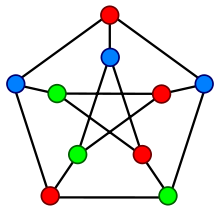
\includegraphics[scale=0.3]{bojene_grafa1}
% 		\caption{Primer ispravnog bojenja cvorova grafa}
% 		\label{bojenje_grafa1}
% 	\end{subfigure}
% 	~
% 	\begin{subfigure}[normla]{0.3\textwidth}
% 		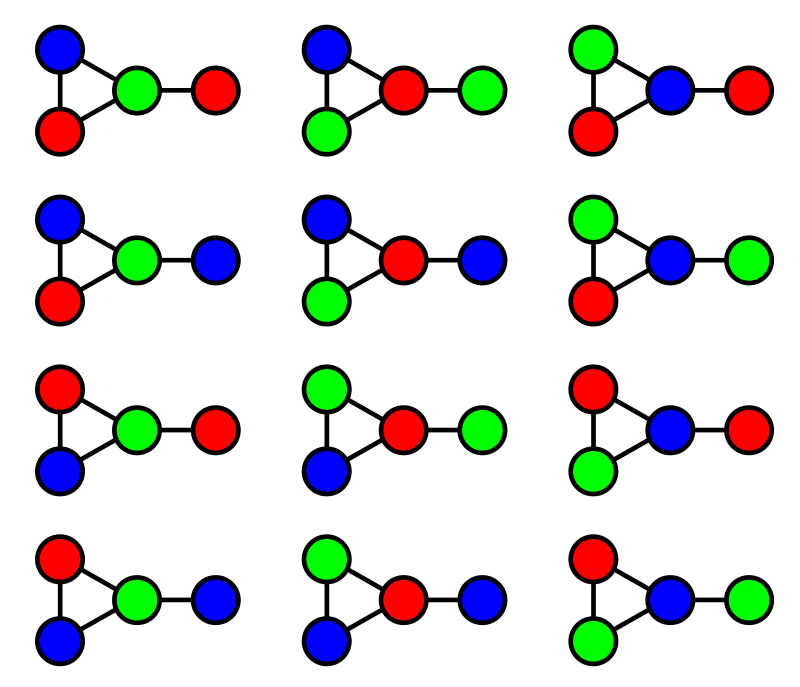
\includegraphics[scale=0.1]{bojenje_grafa2}
% 		\caption{Razlicita ispravna bojenja cvorova grafa}
% 		\label{bojenje_grafa2}
% 	\end{subfigure}
% 		\caption{Slika (a) prikazuje ispravno 3-bojenje Pitersonovog grafa, dok na slici (b) prikazano je 12 razlicitih nacina 3-bojanja grafa. Izvor slika \cite{graph_coloring} }
% \label{bojene_grafa}
% \end{figure}

% \end{frame}


\begin{frame}[fragile]{Bojenje grafa}
  \framesubtitle{Memetski algoritam i njegove primene}

Za neusmeren graf $G = (V, E)$, osnovni memetski algoritam za bojenje grafa ima sledecu formu:
   \begin{itemize}
    \item{Inicijalizacija populacije}
    \item{Kodiranje jedinki}
        \begin{itemize}
            \item Jednu jedinku populacije cini podela skupa $V$ na $k$  disjunktnih podskupova $\{V_1, V_2, ...., V_k\}$
        \end{itemize}
    \item{Lokalna pretraga}
        \begin{itemize}
            \item Tabu pretraga
        \end{itemize}
    \item{Operator ukr�tanja}
        \begin{itemize}
            \item GPX(eng. Greedy Partition Crossover)
        \end{itemize}
    \item{Pravilo a�uriranja populacije}
  \end{itemize}



\end{frame}




\begin{frame}[fragile]{Bojenje grafa}
  \framesubtitle{Memetski algoritam i njegove primene}

   \begin{itemize}
    \item{Hibridni algoritam za bojenje(HCA)}
    \item{Memetski algoritam za bojenje grafa(MACOL)}
    \item{Hibridni evolutivni algoritam u duetu(HEAD)}
  \end{itemize}
  

\end{frame}


\begin{frame}{Kraj}
  \framesubtitle{Memetski algoritam i njegove primene}

  
\centering
\Huge{Hvala na pa�nji!}

\end{frame}




\begin{frame}{Kraj}
  \framesubtitle{Memetski algoritam i njegove primene}
\centering
\Huge{Pitanja?}

\end{frame}




\end{document}